\documentclass[tikz]{standalone}
\usepackage{amsmath}
\usepackage{times}
\usepackage{txfonts}

\usetikzlibrary{arrows}
\usetikzlibrary{intersections}
\usetikzlibrary{math}
\usetikzlibrary{positioning}
\usetikzlibrary{arrows.meta}
\usetikzlibrary{shapes.misc}
\usetikzlibrary{calc}

\begin{document}
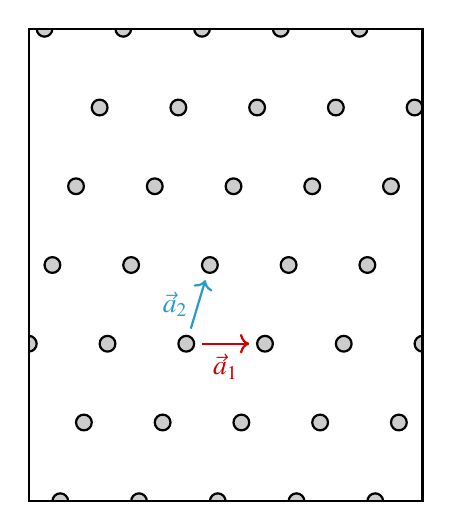
\begin{tikzpicture}[
	dot/.style = {
	  draw, circle, thick, black, fill = gray!40!white,
	  minimum size = 2mm,
	  inner sep = 0pt,
	  outer sep = 1mm,
	},
  ]

  \begin{scope}
	\clip (-2,-2) rectangle (3,4);
	\foreach \y in {-7,-6,...,7} {
	  \foreach \x in {-7,-6,...,7} {
		\node[dot, xshift=3mm*\y] (N\x\y) at (\x, \y) {};
	  }
	}
  \end{scope}
  \draw[black, thick] (-2, -2) rectangle (3,4);

  \draw[red!80!black, thick, ->] 
	(N00) to node[midway, below] {\(\vec{a}_1\)} (N10);
  \draw[cyan!80!black, thick, ->]
	(N00) to node[midway, left] {\(\vec{a}_2\)} (N01);
\end{tikzpicture}
\end{document}
